
% master.tex : master-fil for projektet
% ------------------------------------------------------------------------------
% Dette er hovedfilen for projektet, hvori indhold fra alle input-filer (tekst,
% billeder, litteraturdatabaser, osv.) samles

% Dokumenttypen 'book' er valgt pga. dens mange fleksible indstillinger
% Se https://tex.stackexchange.com/a/36989/118167
\documentclass[11pt, a4paper, twoside, openright, danish, openany]{book}

% Variabler, som bruges til automatisk at indsætte titel, forfattere, osv. på
% forsiden og titelbladet.
\def \projecttitle       {Taylor Polynomier}
\def \projectsubtitle    {og approksimation af funktioner}
\def \projecttheme       {Approksimation af funktioner}
\def \projectdegree      {Matematik} 
\def \projectperiod      {Efterårssemesteret 2020}
\def \projectnumber      {P0}
\def \projectgroup       {B343}
\def \projectauthors     {
  Esben Bonnerup\\
  Kamilla Mattrup\\
  Mikkel Hviid\\
  Martin Nørbjerg
  % ...
}
\def \projectsupervisors {
  Jaron Skovsted Gundersen\\
  % ...
}

% Preamblet indeholder alle de indstillinger og makroer, som skal indsættes for
% hovedindholdet, og i denne skabelon samles det i filen aaumath.sty, som
% definerer en pakke, der kan indlæses med \usepackage.
\usepackage{aaumath}

% Dokumentets indhold indsættes mellem \begin- og \end-makroerne for
% 'document'-blokken
\begin{document}

% Dokumentets 'front matter' tælles ikke med ifm. antal sider og nummereres med
% romerske tal. Herunder hører f.eks. forsiden, titelbladet, forordet og
% indholdsfortegnelsen.
\frontmatter
% incl/misc/frontpage.tex : rapportens forside
% ------------------------------------------------------------------------------


\backgroundsetup{
  scale = 1,
  angle=0,
  opacity=1,
  contents = {
    
\includegraphics[width=\paperwidth,height=\paperheight]{fig/img/aau/waves.pdf}
  }
}
\BgThispage
\pdfbookmark[0]{Forside}{forside}
\begin{titlepage}
  \centering
  \phantom{}
  \vspace{2cm}

  % AAU-segl
  \begin{minipage}[c]{0.2\paperwidth}
    \centering
    \makebox[0pt]{
      % fig/tikz/aau-badge.tex : AAU-logo til forsiden
% ------------------------------------------------------------------------------

\begin{tikzpicture}
  % Tegn hvid cirkel og tilføj det gennemsigtige, blå logo ovenpå
  \node[circle,color=white,fill=white,minimum size=1.175\textwidth] at (0,0) {};
  \node at (0,0) {
\includegraphics[width=\textwidth]{fig/img/aau/logo-circle.pdf}};
\end{tikzpicture}

    }
  \end{minipage}

  % Hovedindhold
  \vspace{4cm}
  {\fontfamily{bch}\selectfont
    \fboxsep0pt\colorbox{white}{
      \begin{minipage}{\textwidth}
        \centering
        \color{AAUblue1}

        \vspace{2em}
        {\Huge\bfseries\projecttitle}

        {\Large\bfseries\projectsubtitle}

        \bigskip
        \parbox{\textwidth}{\centering\large\projectauthors}

        \bigskip
        {\bfseries\large{\projectnumber}-Projekt, Gruppe \projectgroup, \projectdegree}
        \vspace{2em}
      \end{minipage}
    }
  }

\end{titlepage}

% incl/misc/titlepage.tex : rapportens titelblad
% ------------------------------------------------------------------------------
% Titelbladet genereres af makroen \aautitlepage, som er defineret i
% /incl/pre/ext/aautitlepage.sty


\pdfbookmark[0]{Titelblad}{titelblad}
\aautitlepage{
  \projectinfo{
    \projecttitle
  }{
    \projecttheme
  }{
    \projectperiod
  }{
    Gruppe \projectgroup
  }{
    \parbox[t]{\textwidth}{\projectauthors}
  }{
    \parbox[t]{\textwidth}{\projectsupervisors}
  }{
    \today
  }
}{
  \textbf{Institut for Matematiske Fag}\\
  Skjernvej 4A\\
  DK-9220 Aalborg Ø\\
  \href{http://math.aau.dk}{http://math.aau.dk}
}{
  % incl/misc/abstract.tex : projektets abstract
% ------------------------------------------------------------------------------
% Et abstract er et kort resume af rapporten, som vises på titelbladet

}

% incl/misc/contents.tex :
% ------------------------------------------------------------------------------

\pdfbookmark[0]{Indhold}{indhold}

% Indstillingerne i denne fil er grupperet, så de ikke påvirker andre dele
\begingroup

% Slå twoside fra midlertidigt for at undgår sideskift
\makeatletter
\@twosidefalse
\makeatother

% Placer indholdsfortegnelsen på sin egen side (bedst når den kun fylder en side)
\tableofcontents
\clearpage

% Placer oversigtslisterne på efterfølgende sider
%\let\clearpage\relax
%\listoffigures
%\listoftables
%\listofalgorithms
%\lstlistoflistings

\endgroup


% Dokumentets 'main matter' (hovedindhold) er der, hvor det meste indhold skal
% sættes ind. Sider og overskrifter er nummererede med arabiske tal.
\mainmatter

% Input-filer bør opdeles således, at hver fil svarer til et kapitel. Makroen
% \include indsætter et sideskift og indholdet fra den givne stil.

\include{incl/main/introTilTaylorRækker}
\chapter{Introduktion til Taylorpolynomier}
\label{ch:tp}
% Taylorpolynomier
Taylorpolynomier er en måde at approksimere en funktions værdier omkring en værdi $a$, 
approksimationen sker ved hjælp af et $n$'te grads polynomium. Se nedenstående definition: 
\begin{defn}
    Det $n$'te grads Taylorpolynomium $P_n$ til den continuere funktion $f(x)$ omkring værdien $a$ er givet ved:
    \[
    P_n = \sum^{n}_{n=0} \frac{d^n f(a)}{dx^n}\frac{(x-a)^{n}}{n!}
    \]
    hvor $n \in \mathbb{N}$
\end{defn}
\label{def:taylorPolynomium}
Idéen er at polynomiumets $n$'te afledte i $x = a$ bliver det samme som funktionens $n$'te afledte i $x = a$, 
dette skaber en god approksimation omkring $x = a$, men garrentere ikke en god approksimation 
for alle værdier i funktionens definitations mængde: $x \in D(f(x))$. Approksimation bliver dog ofte bedre jo 
flere led Taylorpolynomiet indeholder, dette gælder dog ikke for alle funktioner, hvilket beskrives nærmere i kapitel: \refname{ch:ts}. 
En af fordelene ved at benytte et Taylorpolynomium som approksimation for en mere kompleks funktion
er at polynomier gennerelt er nemmere at integere end andre funktioner, fordi de følger reglen: $\int k x^n = \frac{k}{n + 1}x^{n + 1}$ .

% HUSK MACLAURIN POLYNOMIER

\subsection*{Eksempler på Taylorpolynomier}

\chapter{Restled}

Når man benytter sig af Taylorpolynomier, er det for at approksimere en funktion, og som det ligger i ordet "approksimation", er funktionerne ikke identiske, og der må derfor være en afvigelse fra den oprindelige funktion. Denne afvigelse, også kaldet restleddet eller fejlen, vil vi beskrive i dette afsnit.

\section{Restleddets grundlæggende principper}
\begin{defn}
	I et $n$'tegradspolynomium, $P_n(x)$, kan restleddet, $R_n(x)$, beskrives som 			forskellem mellem funktionen, $f(x)$ som $P_n(x)$ approksimerer, og 		$P_n(x)$.\
	\begin{equation*}
		R_n(x)=|f(x)-P_n(x)|
	\end{equation*}
\end{defn}
Restleddet kan også beskrives på følgende møde:
\begin{equation}
	R_n(x)=\frac{f^{(n+1)}(u)}{(n+1)!}(x-a)^{n+1},
\end{equation}
hvor u er et tal mellem x og a. %plagiat?
\
Man kender sjældent værdien af u, så man kan altså ikke nødvendigvis finde ud af præcis hvor stor afvigelsen er.\\
Man kan dog ofte finde ud af en grænse for, hvor stor restleddet kan være. Med andre ord, kan finde en værdi af $\psi$, der opfylder
\begin{equation}
	|R_n(x)|\leq \psi
\end{equation}
Når man har fundet ud af, at fejlen ikke kan være større end $\psi$, kan man fastlægge et interval 
\begin{equation*}
[P_n(x)-\psi,P_n(x)+\psi],
\end{equation*}
hvori $f(x)$ er indeholdt. I næste afsnit vil et par eksempler på, hvordan dette kan se ud for nogle bestemte funktioner, figurere.\\
Når man sætter restleddet sammen med teorien for Taylor-polynomier, får man Taylors sætning:


\section{Eksempler på anvendelse af restled}
\subsection*{Restleddet anvendt på approksimation af $\sin(x)$}
Vi vil her gennemgå, hvordan man kan approksimere en af de vigtigste konstanter i matematikkens verden, $\sin(\frac{\pi}{2})=1$, ved hjælp af Taylors sætning. Det er måske ikke det mest interresante eksempel, eftersom konstanten 1 er et ret så rationelt tal. Dog kan anvendelsen af restleddet tydeligt demonstreres med dette eksempel.
Som sagt, vil vi gerne approximere $\sin(\frac{\pi}{2})$, og dette gøres ved hjælp af et Maclaurin-polynomium for $\sin(x)$. Mere specifikt benytter vi et Maclaurin-polynomium af tredje orden.
Dette findes ved hjælp af formlen fra \ref{def:taylorPolynomium}, hvor $N=3$ og $a=0$:
\begin{equation}
	P_3=\sum^{3}_{n=0}\frac{x \cdot f^n(0)}{n!}
\end{equation}
\section{Eksempel}
jjgigfji
Som et eksempel vil vi finde restleddet i approksimationen for eksponentialfunktionen.
Vi har tidligere set at Taylor polynomiet for eksponentialfunktionen approksimeret i $x=0$ kan beskrives således:

\[
P_N(x)=\sum^{N}_{n=0}\frac{x^{0}}{0!}+\frac{x^{1}}{1!}+..+\frac{x^{n-1}}{(n-1)!}\frac{x^{n}}{n!}
\]

Vi vælger at kigge på Taylor polynomiet hvor $N=2$:

\[
P_2(x)=\frac{x^{0}}{0!}+\frac{x^{1}}{1!}+\frac{x^{2}}{2!}=1+x+\frac{x^{2}}{2}
\]

Vi vælger x-værdien til at være $1$ og approksimerer:
\[
e^{1}=f(1)\approx P_{2}(1)=1+1+\frac{1^{2}}{2}=\frac{5}{2}=2.5
\]

\[
e^{1}=2.718\approx 2.5
\]

Nu kan vi finde restleddet for approksimationen.
Vi ved at $\frac{d^3}{dx^3}f(x)=e^{x}$ derfor ved vi også at $\frac{d^3}{dx^3}f(s)=e^{s}$ hvor $s$ er et tal mellem 0 og 1. Om $s$-værdien kan vi altså sige at $0<s<1$ da $s<1$ må $e^{s}<e$ da $\frac{d^3}{dx^3}f(s)=e^{s}$ må $\frac{d^3}{dx^3}f(s)<e$.

Restleddet for approksimationen af $e^{x}\approx P_n(x)$ kan beskrives som:
\[
R_N(x)={\frac{e^{s}}{(n+1)!}}\cdot x^{n+1}
\]

\[
R_2(1)<\frac{e}{(2+1)!}\cdot1^{(2+1)}=\frac{e}{6}
\]

Vi ved nu at $f(1)$ ligger i intervallet $(2.5-\frac{e}{6} , 2.5+\frac{e}{6})$. Vi kan ikke sige hvad den eksakte værdi af restleddet er, da vi ikke kender den eksakte værdi af $s$.

\chapter{Taylors sætning anvendt på trigonometriske funktioner og enhedscirklen}
Dette kapitel vil vise, hvordan man anvender den før redegjort for teori på trigonometriske funktioner og enhedscirklen. Målet er at vise, hvordan man numerisk kan udregne værdier for $\sin(x)$, $\cos(x)$ og $\tan(x)$, samt hvordan man kan anvende enhedscirklen og Taylorpolynomier til at tilnærme sig $\pi$.
\section{Taylorrække for $\sin(x)$}
Når man udleder en Taylorrække er det værd at tænke på, hvilken $a$-værdi man vælger, da den ofte afgør, hvor nyttig Taylorrækken er. Målet med Taylorrækken er at gøre $\sin(x)$ nemmere at regne på, så ideelt vil man blandt $\sin(x)$ og dens afledte finde værdier for $a$, der giver heltal eller nemme brøker. Først differentieres $\sin(x)$, så man kan skabe sig et overblik over de afledte til funktionen;
\begin{align*}
f(x) &= \sin(x) \\
f'(x) &= \cos(x) \\
f''(x) &= -\sin(x) \\
f^{(3)}(x) &= -\cos(x) \\
\end{align*}
Sinusfunktionens afledte bliver ved med at svinge mellem positiv og negativ $\sin(x)$ og $\cos(x)$. Hvis man ser på enhedscirklen, så vil funktionerne alle give heltal for hver kvarte omgang, hvilket svarer værdier af $1/2\pi$ ganget med et heltal $z$, hvor $z\in\mathbb{Z}$. Hvis $a=1/2\pi z$, så giver $\sin(x)$ og dens afledte pæne værdier i form af heltallene $-1$, $0$ og $1$. Dog så vil Taylorrækken indeholde $\pi$ for alle $z \neq 0$, hvilket kan gøre udregninger senere svære. Derfor vælges $z=0$ og dermed $a=0$, hvilket giver følgende værdier for $\sin(x)$ og dens afledte;
\begin{align*}
\sin(0) &= 0 \\
\cos(0) &= 1 \\
-\sin(0) &= 0 \\
-\cos(0) &= -1 \\
\end{align*}
Taylorrækken for $\sin(x)$ omkring $0$ bliver derfor;
\begin{align*}
T_{sin} (x) &= 0+x+0 \cdot \frac{x^2}{2}-\frac{x^3}{3!}+0 \cdot \frac{x^4}{4!}+\frac{x^5}{5!}+... 
\\
T_{sin} (x) &= x-\frac{x^3}{3!}+\frac{x^5}{5!}+... \\
\end{align*}
%kilde til ulige funktioners maclaurinrækker
Siden $\sin(x)$ er en ulige funktion, da $\sin(x)=-sin(-x)$, så er $f^{n}(0)=0, \text{hvis} n \mod 2=0$. Dermed er det kun de led, hvor $x$ er opløftet i en ulige eksponent tilbage, hvor eksponenten kan udtrykkes som $2n+1$, for $n\in \mathbb{N}_0$. De resterende led skrifter mellem at være positive $1$ og negative $1$. Her ses det, at leddet $n=0$ er positivt, dermed kan man indfører $(-1)^n$ for at sikre, at leddene skifter mellem at være positive og negative i rigtig rækkefølge. Dermed bliver summen for Taylorrækken for $\sin(x)$ omkring $0$;
\begin{align*}
\sum_{n=0}^{\infty} \frac{(-1)^n}{(2n+1)!}x^{2n+1}
\end{align*}
Der er dog ingen garanti for, at rækken konvergerer med $\sin(x)$. Derfor testes kvotientkriteriet for rækken;
\begin{align*}
\lim\limits_{n \to \infty}
\left\lvert
\frac{\frac{(-1)^{n+1}}{(2(n+1)+1)!}}
{\frac{(-1)^n}{(2n+1)!}} 
\right\lvert
&=
\lim\limits_{n \to \infty}
\left\lvert
\frac{\frac{(-1)^{n+1}}{(2n+3)!}}
{\frac{(-1)^n}{(2n+1)!}}
\right\lvert 
\\
&=
\lim\limits_{n \to \infty}
\frac{\frac{\left\lvert (-1)^{n+1} \right\lvert }{(2n+3)!}}
{\frac{\left\lvert (-1)^n \right\lvert }{(2n+1)!}}
\\
&=
\lim\limits_{n \to \infty}
\frac{\frac{1}{(2n+3)!}}
{\frac{1}{(2n+1)!} }
\\
&=
\lim\limits_{n \to \infty}
\frac{1}{(2n+3)!}
\cdot
\frac{(2n+1)!}{1}
\\
&=
\lim\limits_{n \to \infty}
\frac{1}{(2n+3)(2n+2)}
=0 \\
\end{align*}
Det viser sig, at rækken konvergerer med $\sin(x)$ for alle $x$'er, da $R=\infty$, hvor $R$ er konvergensradiussen.
\begin{equation}\label{eq:sinrække}
\sin(x)=\sum_{n=0}^{\infty} \frac{(-1)^n}{(2n+1)!}x^{2n+1}
\end{equation}
Dette er også Maclaurinrækken for $\sin(x)$, da $c=0$. Med rækken kan man danne Maclaurinpolynomier, hvor der herunder er plottet nogle Maclaurinpolynomiet for at visualisere, hvordan de approksimerer $\sin(x)$;
\begin{figure}[H]
	\centering
	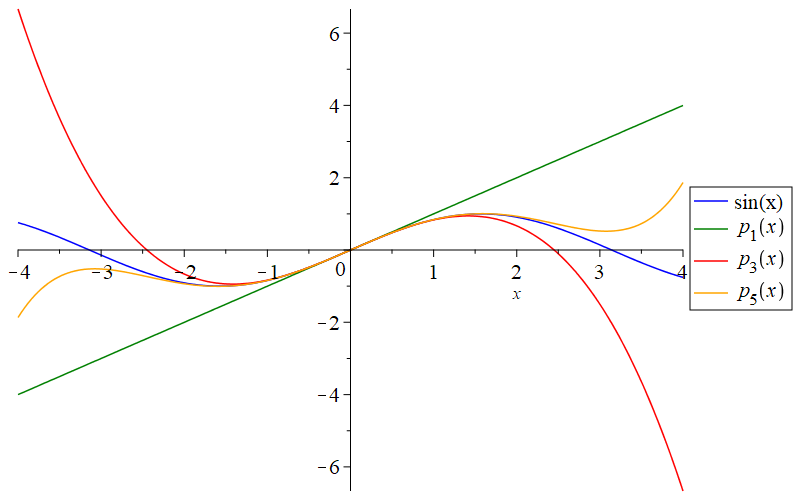
\includegraphics[scale=0.4]{fig/img/taylor_sin}
	\caption{Approksimation af sinus omkring 0 af Maclaurinpolynomier af første, tredje og femte orden}
 	\label{fig:taylor_sin}
\end{figure}
Maclaurinpolynomiet af femte orden kan med god tilnærmelse give værdier for $\sin(x)$ i intervallet $[-\pi /2; \pi /2]$, hvor den absolutte værdi af restleddet maksimalt giver $\left\lvert R_5(\pi/2) \right\lvert = \pi^6/{(6! \cdot 2^6)} = \pi^6/{46080}$. Intervallet dækker en halv svingning, og siden $sin(x)$ svinger harmonisk, så kan man approksimere værdier for $\sin(x)$, der er udenfor intervallet ved at anvende en korresponderende værdi indenfor intervallet. Eksempelvis, så kan man approksimere værdien af $\sin(t)$, hvor $t \in ]\pi/2;\pi]$, ved at udregne $p_5(\pi-t)$, da $\sin(t) = \sin(\pi-t)$. Der er dermed ikke grund til at fremstille et Maclaurinpolynomium af højere orden, da det vil gøre beregningerne sværere.
%referer til eksempel af Esben
\section{Taylorrække for $\cos(x)$}
Hvis man derefter vil udlede en Taylorrække for $\cos(x)$ omkring samme $a$-værdi, så vil man kunne differentiere Taylorrækken for $\sin(x)$, da $\frac{d}{dx}\sin(x)=\cos(x)$. Hvis man differentiere Taylorrækken i ligning \ref{eq:sinrække}, så får man rækken;
%man kan differentiere serien p.ga. teori 19 i calculus-bogen side 536-537 section 9.5
\[
\frac{d}{dx} \sum_{n=0}^{\infty} \frac{(-1)^n}{(2n+1)!}x^{2n+1}
=
\sum_{n=0}^{\infty} \frac{(-1)^n}{(2n)!}x^{2n}
\]
Igen kan man anvende kvotientkriteriet på rækken for at se, om den konvergerer med $\cos(x)$.
\begin{align*}
\lim\limits_{n \to \infty}
\left\lvert
\frac{\frac{(-1)^{n+1}}{(2(n+1))!}}
{\frac{(-1)^n}{(2n)!}} 
\right\lvert
&=
\lim\limits_{n \to \infty}
\left\lvert
\frac{\frac{(-1)^{n+1}}{(2n+2)!}}
{\frac{(-1)^n}{(2n)!}}
\right\lvert 
\\
&=
\lim\limits_{n \to \infty}
\frac{\frac{\left\lvert (-1)^{n+1} \right\lvert }{(2n+2)!}}
{\frac{\left\lvert (-1)^n \right\lvert }{(2n)!}}
\\
&=
\lim\limits_{n \to \infty}
\frac{\frac{1}{(2n+2)!}}
{\frac{1}{(2n)!} }
\\
&=
\lim\limits_{n \to \infty}
\frac{1}{(2n+2)(2n+1)}
=0 \\
\end{align*}
Dermed konvergerer denne række med $\cos(x)$ for alle $x$'er. Rækken er også kendt som Maclaurinrækken for $\cos(x)$;
%evt. kilde til Maclaurinserien for cosinus i bogen side 544-545 section 9.6
\begin{equation}\label{eq:cosrække}
\cos(x)=\sum_{n=0}^{\infty} \frac{(-1)^n}{(2n)!}x^{2n}
\end{equation}
Hvorimod man kunne udlede rækken ved at arbejde med $\cos(x)$, så gjorde de kendte relationer mellem $\cos(x)$ og $\sin(x)$ det nemmere at udlede rækken med den allerede udledte række for $\sin(x)$ i ligning \ref{eq:sinrække}. Maclaurinrækken  for $\sin(x)$ kunne man også integrerer og multiplicerer med $-1$ for at få Maclaurinrækken for $\cos(x)$, da $\int \sin(x) dx=-\cos(x)+k$, hvor $k=-\cos(0)=-1$;
\begin{align*}
-\int \sum_{n=0}^{\infty} \frac{(-1)^n}{(2n)!}x^{2n} dx
&=
-\left(\sum_{n=1}^{\infty} \frac{(-1)^n}{(2n)!}x^{2n}-1\right) \\
-\int \sum_{n=0}^{\infty} \frac{(-1)^n}{(2n)!}x^{2n} dx
&=
\sum_{n=0}^{\infty} \frac{(-1)^n}{(2n)!}x^{2n} \\
\end{align*}
Den samme række opstår, dermed kan man anvende Maclaurinrækken for $\sin(x)$ til at udlede Maclaurinrækken for $\cos(x)$ ved både differentiation og integration. Igen kan man med Maclaurinrækken danne Maclaurinpolynomier;
\begin{figure}[H]
	\centering
	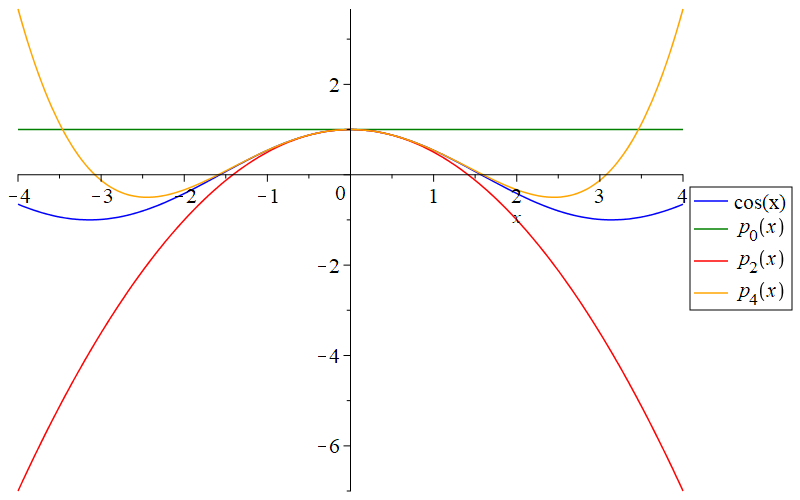
\includegraphics[scale=0.4]{fig/img/taylor_cos}
	\caption{Approksimation af cosinus omkring 0 af Maclaurinpolynomier af nulte, anden og fjerde orden}
 	\label{fig:taylor_cos}
\end{figure}
Mangen til \ref{fig:taylor_sin}, så ses det, at Maclaurinpolynomiet af fjerde orden giver en god tilnærmelse af $\cos(x)$ i intervallet $[-\pi /2; \pi /2]$, hvor den maksimale absolutte værdi af restleddet er $\left\lvert R_4(\pi/2) \right\lvert = \pi^5/(5! \cdot 2^5) = \pi^5/3840$. $[-\pi /2; \pi /2]$ dækker et udsving af $\cos(x)$, hvilket man kan anvende til at finde værdier for $\cos(x)$ udover intervallet, igen mangen til Maclaurinpolynomiet af femte orden for $\sin(x)$.
\section{Approksimation af $\tan(x)$}
Til $\tan(x)$ kan man igen udnytte dens relation til de andre trigonometriske funktioner, hvor ligningen $\tan(x)=\frac{\sin(x)}{\cos(x)}$ er gældende. Hvis man derfor tager rækken i ligning \ref{eq:sinrække} og dividerer med rækken i ligning \ref{eq:cosrække}, så får man $\tan(x)$;
\begin{equation}\label{eq:tanbrøk}
\tan(x)
=
\frac{\sum_{n=0}^{\infty} \frac{(-1)^n}{(2n+1)!}x^{2n+1}}
{\sum_{n=0}^{\infty} \frac{(-1)^n}{(2n)!}x^{2n}}
\end{equation}
Hvis man tager delsumme af de to summe med samme øvre grænse, så for man en rationel funktion, som approksimerer $\tan(x)$ omkring $0$;
\begin{figure}[H]
	\centering
	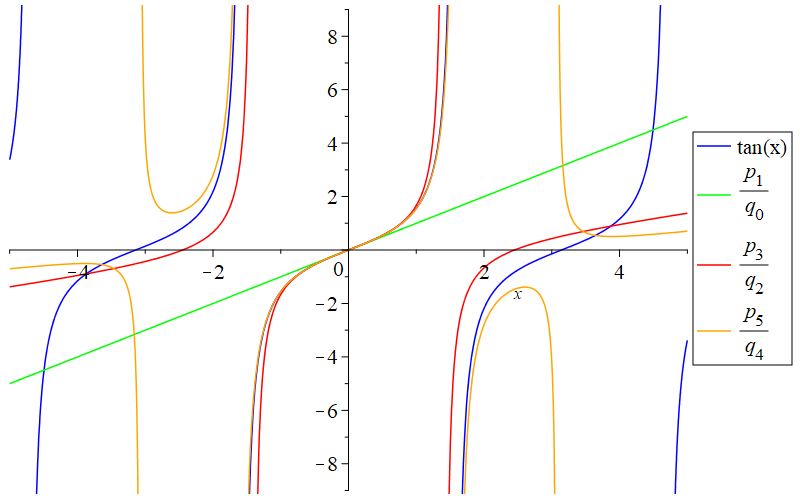
\includegraphics[scale=0.4]{fig/img/approks_tan}
	\caption{Approksimation af tangens omkring 0 via Maclaurinpolynomier af $\sin(x)$, noteret $p_n$, og $\cos(x)$, noteret $q_n$.}
 	\label{fig:approks_tan}
\end{figure}
Approksimationen af tangens går igen tilbage til Maclaurinpolynomierne på \ref{fig:taylor_sin}, da de rationelle funktioner på \ref{fig:approks_tan} kan omformuleres til $R(x)=p_n(x)/p_n'(x)$. Omformuleringen giver også god mening i forhold til gennemgangen, hvor Maclaurinrækken for $\cos(x)$ blev udledt ved at differentiere Maclaurinrækken for $\sin(x)$, så $\tan(x)=\sin(x)/\frac{d}{dx}\sin(x)$. Derfor kan man med et Maclaurinpolynomium for $\sin(x)$ approksimere $\tan(x)$ omkring $0$.
\section{Approksimation af $\pi$}
Taylorpolynomier kan også anvendes, når man skal bestemme en værdi numerisk. En sådan værdi kunne være $\pi$, hvor man anvender, hvordan $\pi$ hænger sammen med andre størrelser i cirkler. En sammenhæng er arealet af en cirkel og radiussen; $A=\pi \cdot r^2$. Her kan man med fordel vælge $r=1$, så $A=\pi$ og cirklen har ligningen $x^2+y^2=1$. Ligningen kan ændres, så man får en funktion over en halvcirkel; $y=g(x)=\sqrt{1-x^2}$. Arealet under funktionen er $\pi/2$, men det er svær at integrere $g(x)$, derfor dannes et Taylorpolynomium over funktionen, og det integreres i stedet for $g(x)$. Til denne funktion og dens afledte findes de pæneste værdier, når $x=0$.
\begin{align*}
g(0) &= 1 \\
g'(0) &= 0 \\
g''(0) &= -1 \\
g^{(3)}(0) &= 0 \\
g^{(4)}(0) &= -3 \\
\end{align*}
Dermed kan man lave et fjerdeordens Maclaurinpolynomium.
\begin{align*}
p_{4} (x) &= 1 + 0\cdot \frac{x}{1!} - 1\cdot \frac{x^2}{2!} + 0\cdot \frac{x^3}{3!} - 3\cdot \frac{x^4}{4!}
\\
p_{4} (x) &= 1-\frac{x^2}{2}-\frac{x^4}{8} \\
\end{align*}
Maclaurinpolynomiet integreres fra $x=-1$ til $x=1$, da funktion, og dermed halvcirklen, er defineret i intervallet [-1;1].
\[
\int_{-1}^{1} 1-\frac{x^2}{2}-\frac{x^4}{8} dx = \frac{97}{60} \approx 1,6167
\]
Resultatet var en tilnærmelse af $\pi/2$, så $2\cdot 1,6167 = 3,2334$ er en tilnærmelse af $\pi$. Tilnærmelsen er dog kun med $1$ korrekt ciffer og ingen korrekte decimaler. 
Hvis der ønskes en bedere approksimation bør antallet af led i taylor polynomiet stige, dette er 
imidlertidigt ikke særligt simpelt at lave i hånden da de afledte hurtigt vokser i kompleksitet, 
se appendix (\ref{app:afledte}).  % REFERE TIL APPENDIX
Derfor blev der udarbejdet et simpelt python program til beregningerne, 
som kunne beregne de afledte op til $n$'te orden og derefter integrere taylor polynomiet:
Kildekoden kan ses i appendix (\ref{app:kildeKode}). 
Koden indeholder 2 hoved funktioner:
\begin{itemize}
  \item "computeDerivatives" som beregner de afledte for funktionen $f(x)$ 
  i punktet $a$, dette sker ved hjælp af python pakken SymPy, herefter returneres disse som en liste af værdier.  
  \item "intergrateTaylor" som beregner værdien af intergralet imellem to endepunkter
  og returnere værdierne for intergralet $\int_{-1}^1 P_N (x) dx$ ved specifike ordener $N$. 
\end{itemize}
Når koden køres fås følgende værdier:
\begin{table}[H]
  \begin{center}
    \begin{tabular}{ |c|c|c|c|c|c|c| }
      \hline
        Antal led $N$ & 10 & 20 & 50 & 100 & 200 & 500 \\
      \hline
        Approksimation & $1.5852$ & $1.5763$ & $1.5723$ & $1.5713$ & $1.5709$ & $1.5708$ \\
      \hline
    \end{tabular}
    \caption{Approksimationen i forhold til ordenen af taylor polynomiet}
  \end{center}
\end{table}
%\label{tab:approksimationenVsN}
Som det kan ses i tabellen sker der en mindre og mindre ændring i værdien for approksimationen når $N$ bliver større og større
I denne sammenhæng er det også interessant at kigge på fejlen imellem approksimationen $\int_{-1}^1 P_N(x) dx$ og $\frac{\pi}{2}$:
\begin{figure}[H]
  \centering
  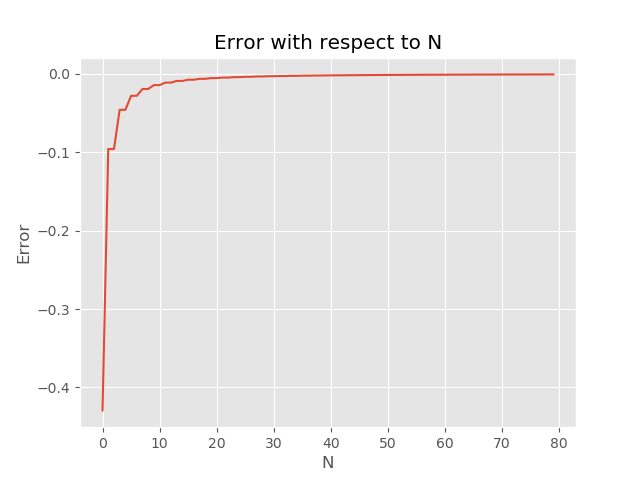
\includegraphics[width=\textwidth]{fig/img/ErrorWithRespectToN.png}
  \caption{Fejl i forhold til antalet af led $N$}
  \label{fig:FejlIForholdTilN}
\end{figure}
Som det kan ses falder fejlen hurtigt i starten når $N$ er lille, men som $N$ vokser flader fejlen ud fordi $P_{N-1}(x) \approx P_{N}(x)$ når $N \rightarrow \infty$.

\lstinputlisting[
  firstline=1,
  lastline=33,
  label={code:pi},
  caption={Approximation af pi ved hjælp af python}
]{source/pi.py}
Koden indeholder 2 specielle funktioner:
\begin{itemize}
  \item "computeDerivatives" som beregner de afledte for funktionen f 
  i punktet a, dette sker ved hjælp af python pakken SymPy, herefter returneres disse som en liste af værdier.  
  \item "intergrateTaylor" som beregner værdien af intergralet imellem to endepunkter i et interval
  og returnere værdierne for intergralet ved specifike ordener. 
\end{itemize} 
Når koden køres fåes følgende værdier:
\begin{center}
  \begin{tabular}{ |c|c|c|c|c|c|c| }
    \hline
      Antal led $n$ & 10 & 20 & 50 & 100 & 200 & 500 \\
    \hline
      Approximation & $1.5852$ & $1.5763$ & $1.5723$ & $1.5713$ & $1.5709$ & $1.5708$ \\
    \hline
  \end{tabular}
\end{center}
%\label{tab:approksimationenVsN}
Som det kan ses i tabellen sker der en mindre og mindre ændring i værdien for approksimationen når n bliver større og større
I denne sammenhæng er det også intresant at kigge på fejlen $R$ imellem approksimationen og $\frac{\pi}{2}$:
\begin{figure}[H]
  \centering
  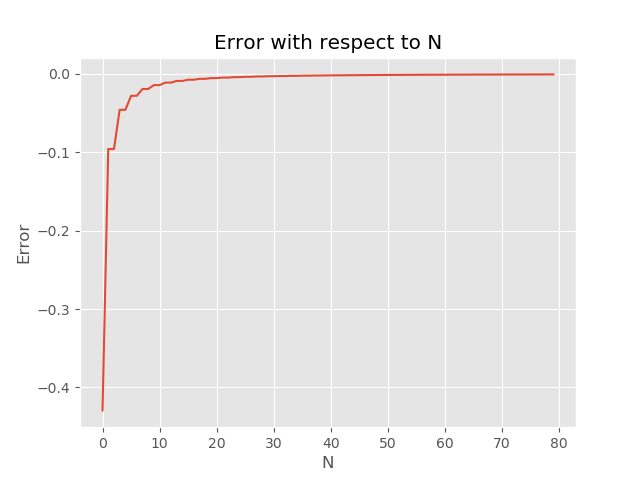
\includegraphics[width=\textwidth]{fig/img/ErrorWithRespectToN.png}
  \caption{Fejl i forhold til antalet af led $n$}
  \label{fig:FejlIForholdTilN}
\end{figure}
Som det kan ses falder fejlen hurtigt i starten når $n$ er lille, men som $n$ vokser flader funktionen ud.

% \include{incl/main/example2}
% ...

% Appendicer indsættes inde i en appendices-blok og bliver nummereret med
% bogstaver i stedet for tal
\begin{appendices}
  \chapter{De afledte af $\sqrt{1-x^2}$}
\label{app:afledte}
De afledte til $g(x)$, differentieret med kædereglen og produktreglen;
\begin{align*}
g(x) &= \sqrt{1-x^2} \\
\end{align*}
\begin{align*}
g'(x) &= \frac{1}{2\sqrt{1-x^2}} (-2x)\\
&= \frac{-x}{\sqrt{1-x^2}} \\
\end{align*}
\begin{align*}
g''(x) &= \frac{-1}{\sqrt{1-x^2}} -x\left(\frac{-1}{2}\right)(-2x)\frac{1}{\sqrt{1-x^2}(1-x^2)}\\
&= \frac{-1}{\sqrt{1-x^2}} -\frac{x^2}{\sqrt{1-x^2}(1-x^2)}\\
&= \frac{-1}{\sqrt{1-x^2}}\left(\frac{x^2}{1-x^2}+1\right)\\
\end{align*}
\begin{align*}
g^{(3)}(x) &= \frac{-x}{\sqrt{1-x^2}(1-x^2)}\left(\frac{x^2}{1-x^2}+1\right)- \frac{1}{\sqrt{1-x^2}}\left(\frac{2x}{1-x^2}+\frac{2x^3}{(1-x^2)^2}\right)\\
&= \frac{-1}{\sqrt{1-x^2}}\left(\frac{x^3}{(1-x^2)^2}+\frac{x}{1-x^2}\right)- \frac{1}{\sqrt{1-x^2}}\left(\frac{2x}{1-x^2}+\frac{2x^3}{(1-x^2)^2}\right)\\
&=\frac{-1}{\sqrt{1-x^2}}\left(\frac{3x^3}{(1-x^2)^2}+\frac{3x}{1-x^2}\right) \\
\end{align*}
\begin{align*}
g^{(4)}(x) &= \frac{-x}{\sqrt{1-x^2}(1-x^2)}\left(\frac{3x^3}{(1-x^2)^2}+\frac{3x}{1-x^2}\right)-\frac{1}{\sqrt{1-x^2}}\left(\frac{9x^2}{(1-x^2)^2}+\frac{12x^4}{(1-x^2)^3}+\frac{3}{1-x^2}+\frac{6x^2}{(1-x^2)^2}\right) \\
&= \frac{-1}{\sqrt{1-x^2}}\left(\frac{3x^4}{(1-x^2)^3}+\frac{3x^2}{(1-x^2)^2}\right)-\frac{1}{\sqrt{1-x^2}}\left(\frac{9x^2}{(1-x^2)^2}+\frac{12x^4}{(1-x^2)^3}+\frac{3}{1-x^2}+\frac{6x^2}{(1-x^2)^2}\right) \\
&= \frac{-1}{\sqrt{1-x^2}} \left(\frac{15x^4}{(1-x^2)^3}+\frac{18x^2}{(1-x^2)^2}+\frac{3}{1-x^2}\right)\\
\end{align*}
  \include{incl/app/kildeKode}
  % ..
\end{appendices}

% Dokumentets 'back matter' er til ekstra ting som f.eks. litteraturlisten.
% Overskrifter bliver ikke nummereret her.
\backmatter

% Automatisk litteraturliste baseret på, hvilke kilder, der er blevet refereret
% til i løbet af rapporten.
\bibliographystyle{apalike}
\bibliography{
  incl/bib/books,
  incl/bib/articles,
  incl/bib/software
}

\end{document}
